\documentclass{article}
\usepackage[utf8]{inputenc}
\usepackage{graphicx}
\usepackage{hyperref}
\usepackage{geometry}
\usepackage{enumitem}
\usepackage{xcolor}
\usepackage{listings}
\usepackage{array}

\geometry{a4paper, margin=1in}

\title{Secure P2P Chat Application with Video Calling}
\author{}
\date{}

% Rest of your preamble remains unchanged
\definecolor{codegreen}{rgb}{0,0.6,0}
\definecolor{codegray}{rgb}{0.5,0.5,0.5}
\definecolor{codepurple}{rgb}{0.58,0,0.82}
\definecolor{backcolour}{rgb}{0.95,0.95,0.92}

\lstdefinestyle{mystyle}{
    backgroundcolor=\color{backcolour},   
    commentstyle=\color{codegreen},
    keywordstyle=\color{magenta},
    numberstyle=\tiny\color{codegray},
    stringstyle=\color{codepurple},
    basicstyle=\ttfamily\footnotesize,
    breakatwhitespace=false,         
    breaklines=true,                 
    captionpos=b,                    
    keepspaces=true,                 
    numbers=left,                    
    numbersep=5pt,                  
    showspaces=false,                
    showstringspaces=false,
    showtabs=false,                  
    tabsize=2
}

\lstset{style=mystyle}

\begin{document}

\begin{center}
    
\includegraphics[width=1\textwidth]{Logo.png} \\ % Reduced width for better proportions
    \vspace{0.5cm}
    
    {\LARGE\bfseries Secure P2P Chat Application with Video Calling}
    \vspace{1cm}
    
    % Instructor information - corrected tabular
    \begin{tabular}{l@{\hspace{1cm}}r}
        \textbf{Instructor:} & Prof. Tamal Das \\
        \textbf{Course:} & Computer Networks \\
        \textbf{Date:} & \today \\
    \end{tabular}
    
    \vspace{1cm}
    
    \textbf{\Large Team Members}
    \vspace{0.5cm}
    
    \begin{tabular}{@{}lr@{}}
        \hline
        \textbf{Name} & \textbf{ID Number} \\
        \hline
        HARISH R & 220010018 \\
        RICKY ROY RAGOLU & 220010047 \\
        SHIVAPRASAD F. N. & 220010054 \\
        SIDDHARTH BALAI & CE23BT007 \\
        KAILAS S & MC23BT022 \\
        \hline
    \end{tabular}
\end{center}

\vspace*{2cm} % Add space before main content

\maketitle

\section*{Introduction}

Our Secure Peer-to-Peer Chat App is a private messaging tool that lets people communicate directly without using any central servers. Unlike regular chat apps that store your messages on company servers, our system keeps everything between you and the person you're talking to.

Key features include:

\begin{itemize}
    \item \textbf{Private messaging}: All texts are locked with strong encryption that only you and your friend can open.
    \item \textbf{File sharing}: Send documents and photos securely, which automatically save to a "Downloads" folder.
    \item \textbf{Video calls}: Make face-to-face calls that stay private.
\end{itemize}

We built this because everyone deserves simple, private communication without worrying about who might be watching. The app runs on most computers and doesn't require special hardware or expensive subscriptions. Everything stays between you and your chat partners - no middleman, no data collection, and no hidden tracking.

\section*{Motivation}
In an era of increasing digital communication and privacy concerns, we recognized the need for a secure, decentralized communication platform that doesn't rely on central servers. Our motivation was to create a private, peer-to-peer chat solution with end-to-end encryption that also supports rich media features like file sharing and video calls.

\section*{Goals}
\begin{itemize}
    \item Create a completely decentralized chat application
    \item Implement strong end-to-end encryption for all communications
    \item Support text messaging, file transfers, and video calls
    \item Automatically discover peers on the local network
    \item Ensure user-friendly operation with clear command interface
\end{itemize}

\newpage
\section*{Tech Stack}
\begin{table}[h]
\centering
% \caption{Technology Stack Overview}
\label{tab:techstack}
\begin{tabular}{|l|l|p{8cm}|}
\hline
\textbf{Category} & \textbf{Technology} & \textbf{Description} \\ \hline
Programming Language & Python 3 & Primary language for the entire application \\ \hline
Cryptography & \texttt{cryptography} library & RSA-2048 with OAEP padding for end-to-end encryption \\ \hline
Networking & Python \texttt{socket} & TCP for encrypted messaging, UDP for peer discovery \\ \hline
Video Processing & OpenCV & Video capture, compression, and display \\ \hline
Audio Processing & sounddevice & Audio capture and playback \\ \hline
Data Processing & numpy & Handling audio/video data streams \\ \hline
Logging & Python \texttt{logging} & System activity and error logging \\ \hline
File Handling & Python \texttt{os}, \texttt{hashlib} & Secure file transfers with SHA-256 verification \\ \hline
\end{tabular}
\end{table}

\begin{lstlisting}[language=Python]
import socket
import threading
import time
import os
import hashlib
import json
from datetime import datetime
import logging
from cryptography.hazmat.primitives.asymmetric import rsa, padding
from cryptography.hazmat.primitives import serialization, hashes
from cryptography.hazmat.backends import default_backend
import sys
import select
import cv2  # OpenCV used for video capture and display
import numpy as np  # For converting image bytes to numpy array
import sounddevice as sd
\end{lstlisting}

\section*{Key Features Implemented}
\subsection*{1. Secure Peer Discovery}
\begin{itemize}
    \item Uses UDP broadcast on port 37020 to discover peers on the local network
    \item Each peer broadcasts their username, IP, listening port, and public key
    \item Automatically maintains a list of available peers
\end{itemize}

\subsection*{2. End-to-End Encryption}
\begin{itemize}
    \item RSA 2048-bit asymmetric encryption for all messages
    \item OAEP padding with SHA-256 for secure encryption
    \item Public key exchange during connection establishment
    \item Key verification to prevent man-in-the-middle attacks
    \item \textbf{Wireshark Verification}: Our network captures confirm all peer-to-peer communications are fully encrypted.
    \item \textbf{Traffic Analysis}: Wireshark monitoring shows the expected protocol behavior - UDP broadcasts for discovery followed by encrypted TCP streams for messaging, file transfers, and video calls, with no sensitive data exposed in transit.

    \begin{figure}[h]
        \centering
        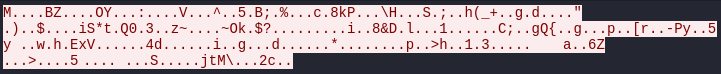
\includegraphics[width=0.85\textwidth]{wireshark.png}
        \caption{Wireshark analysis showing encrypted payloads}
    \end{figure}
\end{itemize}

\subsection*{3. Encrypted Communication Channels}
\begin{itemize}
    \item All text messages are encrypted before transmission
    \item File transfers are protected with:
    \begin{itemize}
        \item Encrypted metadata (filename, size, hash)
        \item SHA-256 hash verification for file integrity
        \item Automatic creation of \texttt{downloads} directory on the receiver's side if it doesn't exist
    \end{itemize}
\end{itemize}

\subsection*{4. Video Calling}
\begin{itemize}
    \item Bidirectional video streaming using OpenCV
    \item Audio streaming with sounddevice library
    \item Separate UDP ports for video and audio streams
    \item Quality compression with JPEG encoding for video
\end{itemize}

\subsection*{5. Logging System}
\begin{itemize}
    \item Comprehensive logging to \texttt{p2p\_chat.log}
    \item Records peer discovery, connection events, and errors
    \item Helps with debugging and monitoring network activity
\end{itemize}


\section*{Encryption Implementation Details}
The application uses RSA-2048 with OAEP padding for all secure communications. Here's how it works:

\begin{lstlisting}[language=Python]
# Key Generation:
private_key = rsa.generate_private_key(
    public_exponent=65537,
    key_size=2048,
    backend=default_backend()
)
public_key = private_key.public_key()

# Message Encryption:
encrypted_msg = public_key.encrypt(
    message.encode('utf-8'),
    padding.OAEP(
        mgf=padding.MGF1(algorithm=hashes.SHA256()),
        algorithm=hashes.SHA256(),
        label=None
    )
)

# Message Decryption:
decrypted_msg = private_key.decrypt(
    encrypted_msg,
    padding.OAEP(
        mgf=padding.MGF1(algorithm=hashes.SHA256()),
        algorithm=hashes.SHA256(),
        label=None
    )
).decode('utf-8')
\end{lstlisting}

All network traffic except the initial peer discovery broadcasts are encrypted. The log file (\texttt{p2p\_chat.log}) records connection events but never stores message content or encryption keys.

\section*{File Transfer Implementation}
When receiving files, the application automatically creates a \texttt{downloads} directory if it doesn't exist:

\begin{lstlisting}[language=Python]
# Create downloads directory if it doesn't exist
os.makedirs('downloads', exist_ok=True)
filepath = os.path.join('downloads', filename)

# Receive file content in chunks
hasher = hashlib.sha256()
received = 0
with open(filepath, 'wb') as f:
    while received < filesize:
        chunk = self.peer_socket.recv(min(4096, filesize - received))
        if not chunk:
            break
        f.write(chunk)
        hasher.update(chunk)
        received += len(chunk)
\end{lstlisting}

\section*{Setup Instructions}
\subsection*{Prerequisites}
\begin{itemize}
    \item Python 3.7 or higher
    \item Required libraries: \texttt{cryptography}, \texttt{opencv-python}, \texttt{sounddevice}, \texttt{numpy}
\end{itemize}

\subsection*{Installation}
\begin{enumerate}
    \item Clone the repository
    \item Install dependencies:
    \begin{lstlisting}[language=bash]
    pip install cryptography opencv-python sounddevice numpy
    \end{lstlisting}
    \item Run the application:
    \begin{lstlisting}[language=bash]
    python p2p_chat.py [username] OR python3 p2p_chat.py [username]
    \end{lstlisting}
\end{enumerate}

\subsection*{Usage}
\begin{enumerate}
    \item Start the application with a unique username
    \item Discover peers automatically on your local network
    \item Use commands:
    \begin{itemize}
        \item \texttt{/help} - To see commands
        \item \texttt{/connect [username]} - Connect to a peer
        \item \texttt{/msg [message]} - Send encrypted message
        \item \texttt{/sendfile [path]} - Send encrypted file (will be saved in receiver's \texttt{downloads} folder)
        \item \texttt{/videocall} - Start video call
        \item \texttt{/disconnect} - End current connection
        \item \texttt{/exit} - Quit application
    \end{itemize}
\end{enumerate}

\section*{Demonstration Video}
\href{https://youtu.be/example-link}{Click here to view the demonstration video}.

The video demonstrates:
\begin{itemize}
    \item Peer discovery and connection establishment
    \item Encrypted text messaging
    \item Secure file transfer (including automatic \texttt{downloads} folder creation)
    \item Video call initiation and operation
    \item Network behavior visible in Wireshark (encrypted traffic)
\end{itemize}

\section*{Security Considerations}
\begin{itemize}
    \item All communications are end-to-end encrypted
    \item Public keys are verified during connection
    \item No central server means no single point of failure
    \item File transfers include hash verification
    \item Video/audio streams use separate UDP ports
    \item Downloaded files are saved in a dedicated \texttt{downloads} directory
\end{itemize}

\section*{Future Enhancements}
\begin{itemize}
    \item Group chat functionality
    \item Message history with local encryption
    \item Better video compression and quality adjustment
    \item NAT traversal for internet-wide communication
    \item Mobile client support
    \item Configurable download directory location
\end{itemize}

This application provides a secure, private communication platform that respects user privacy while offering rich media features, all without relying on any central infrastructure. The automatic creation of the \texttt{downloads} directory ensures a seamless file transfer experience for users.

\end{document}
